\chapter{Result}
This chapter presents the results of the conducted evaluation. Appendix \ref{appendix:raw} contains raw data and metrics over data that may not be shown in this chapter. The chapter starts with presenting the results from the \textit{\nameref{Performance}} evaluations where the parameters time and memory is measured. Next and the last section is \textit{\nameref{Applications}} where Java applications have been evaluated measuring security vulnerabilities with and without Dynamic Taint Propagation.



\section{Applications}
\label{Applications}
The presented results in this section are from evaluating Java applications for security vulnerabilities with and without dynamic taint tracking. The results from each application are listed in its table where vulnerability type and the number of vulnerabilities are listed. In the presentation of the result in the text are vulnerabilities of the same type aggregated. By aggregating all four average prevention rates do we get that the overall prevention rate for the applications is 81\%.

Table \ref{table:MicroTable} shows the vulnerabilities from evaluating Stanford SecuriBench Micro \parencite{securiBenchMicro}. In the table can we see that the most common vulnerability is reflected Cross-Site Scripting where 71 vulnerabilities are present. Second most common is SQL Injection with 20 and the least common with one vulnerability is Buffer Overflow. By enabling dynamic taint tracking on the Stanford SecuriBench Micro \parencite{securiBenchMicro} application results in a 100\% prevention rate.

\begin{table}[H]
  \centering
  \caption{Security Vulnerabilities Detected by Dynamic Taint Tracker (DTT) in Stanford SecuriBench Micro}
  \label{table:MicroTable}
    \begin{tabular}{rcc}
      & \textbf{Vulnerabilities} & \textbf{Found by DTT} \\
      \textbf{Cross-Site Scripting (Reflected)} & 71            & 71  \\
      \textbf{SQL Injection}                    & 20            & 20  \\
      \textbf{Buffer Overflow}                  & 1             & 1  
    \end{tabular}
\end{table}

Table \ref{table:InsecureTable} shows the vulnerabilities from running InsecureWebApp \parencite{insecure} with and without Dynamic Taint Tracker. Of the two types of vulnerabilities is SQL Injection the first with six vulnerabilities and reflected Cross-Site Scripting with two. Enabling dynamic taint tracking on InsecureWebApp \parencite{insecure} results in 100\% prevention rate on SQL Injection attacks and 0\% for Cross-Site Scripting. The overall prevention rate is 75\%. 

\begin{table}[H]
  \centering
  \caption{Security Vulnerabilities Detected by Dynamic Taint Tracker (DTT) in InsecureWebApp}
  \label{table:InsecureTable}
    \begin{tabular}{rcc}
      & \textbf{Vulnerabilities} & \textbf{Found by DTT} \\
      \textbf{Cross-Site Scripting (Reflected)}      & 2             & 0  \\
      \textbf{SQL Injection - Authentication Bypass} & 2             & 2  \\
      \textbf{SQL Injection - Hypersonic SQL}        & 4             & 4  
    \end{tabular}
\end{table}

The results from evaluating the application SnipSnap \parencite{snipsnap} is seen in Table \ref{table:SnipSnapTable}. In this table can we see that the most common vulnerability is reflected Cross-Site Scripting with 172 occurrences. Second Largest is SQL Injection with 49 occurrences followed by CRLF Injection with two. Enabling dynamic taint tracking yields an overall prevention rate of 77.2\%. All CRLF Injection is prevented. Cross-Site Scripting prevented with 77.3\% and SQL Injection with 75.5\%.

\begin{table}[H]
  \centering
  \caption{Security Vulnerabilities Detected by Dynamic Taint Tracker (DTT) in SnipSnap}
  \label{table:SnipSnapTable}
  \begin{tabular}{rcc}
    & \textbf{Vulnerabilities} & \textbf{Found by DTT} \\
    \textbf{Cross-Site Scripting (Reflected)}      & 172           & 133  \\
    \textbf{CRLF Injection}                        & 3             & 3    \\
    \textbf{SQL Injection}                         & 47            & 37   \\
    \textbf{SQL Injection - Authentication Bypass} & 2             & 0       
  \end{tabular}
\end{table}

Table \ref{table:Ticketbook} shows the vulnerabilities from evaluating Ticketbook \parencite{ticketbook}. The most common vulnerability was Cross-Site Scripting with 14 occurrences. SQL Injection was the least with one. The prevention rate of SQL Injection was 100\% and for Cross-Site Scripting 71.4\%. The overall prevention rate is 73.3\%.

\begin{table}[H]
  \centering
  \caption{Security Vulnerabilities Detected by Dynamic Taint Tracker (DTT) in Ticketbook}
  \label{table:Ticketbook}
  \begin{tabular}{ccc}
    & \textbf{Vulnerabilities} & \textbf{Found by DTT} \\
    \textbf{Cross-Site Scripting (Persistent)} & 2             & 2 \\
    \textbf{Cross-Site Scripting (Reflected)}  & 12            & 8 \\
    \textbf{SQL Injection}                     & 1             & 1
  \end{tabular}
\end{table}



\section{Performance Overhead}
\label{Performance}
The results from benchmarking the application on DaCapo Benchmark Suit \parencite{dacapo} is seen in Figure \ref{fig:Time} and \ref{fig:Memory}. Both graphs are constructed to show the added overhead of running the applications with dynamic taint tracking activated. The graphs are constructed based on the data in Table \ref{TimeTable} and \ref{MemoryTable}.



\subsection{Time}
Figure \ref{fig:Time} displays the results of the average time overhead per application. The results show that the application with the least average time overhead was Tradesoap where 14.7\% was added. The largest application, however, was Batik with an overhead of 432.2\%. The average overall is 162.9\%.

\begin{figure}[H]
    \centering
    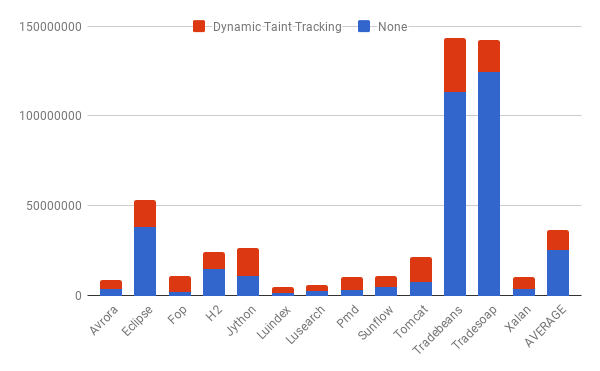
\includegraphics[width=\textwidth]{images/Time.png}
    \caption{Average Added Time in Microseconds}
    \label{fig:Time}
\end{figure}



\subsection{Memory}
Figure \ref{fig:Memory} displays the results of the average memory overhead per application. The results show that the application with the least average memory overhead was Eclipse where 5.5\% was added. The largest application, however, was Batik with an overhead of 344.6\%. The average overall is 142.7\%.

\begin{figure}[H]
    \centering
    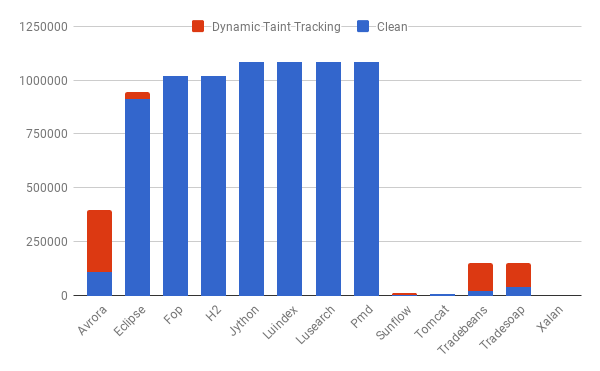
\includegraphics[width=\textwidth]{images/Memory.png}
    \caption{Average Added Memory in Kilobytes}
    \label{fig:Memory}
\end{figure}